\documentclass[a4paper,12pt]{article}

\usepackage{amsmath, amssymb, amsthm}
\usepackage{geometry}
\geometry{margin=1in}
\usepackage{graphicx}
\usepackage{hyperref}
\usepackage{xcolor}
\usepackage{enumitem}
\usepackage{listings}
\usepackage{float}
\usepackage{array}
\usepackage{placeins}
\usepackage{enumitem}
\usepackage{listings}
\usepackage{tikz}
\usepackage{amsmath}    
\usepackage{booktabs}
\usepackage{tabularx}
\usepackage{subcaption}


\title{Linear Regression}
\author{Christian Darvin}
\date{\today}

\begin{document}

\maketitle
\tableofcontents

\newpage

\section{Linear Regression}
A statistical technique used to find the relationship between \textbf{features} and a \textbf{label}. Possible correlations: \textbf{Positive, Negative, Non-linear, No Correlation}.
\begin{figure}[H]
    \centering
    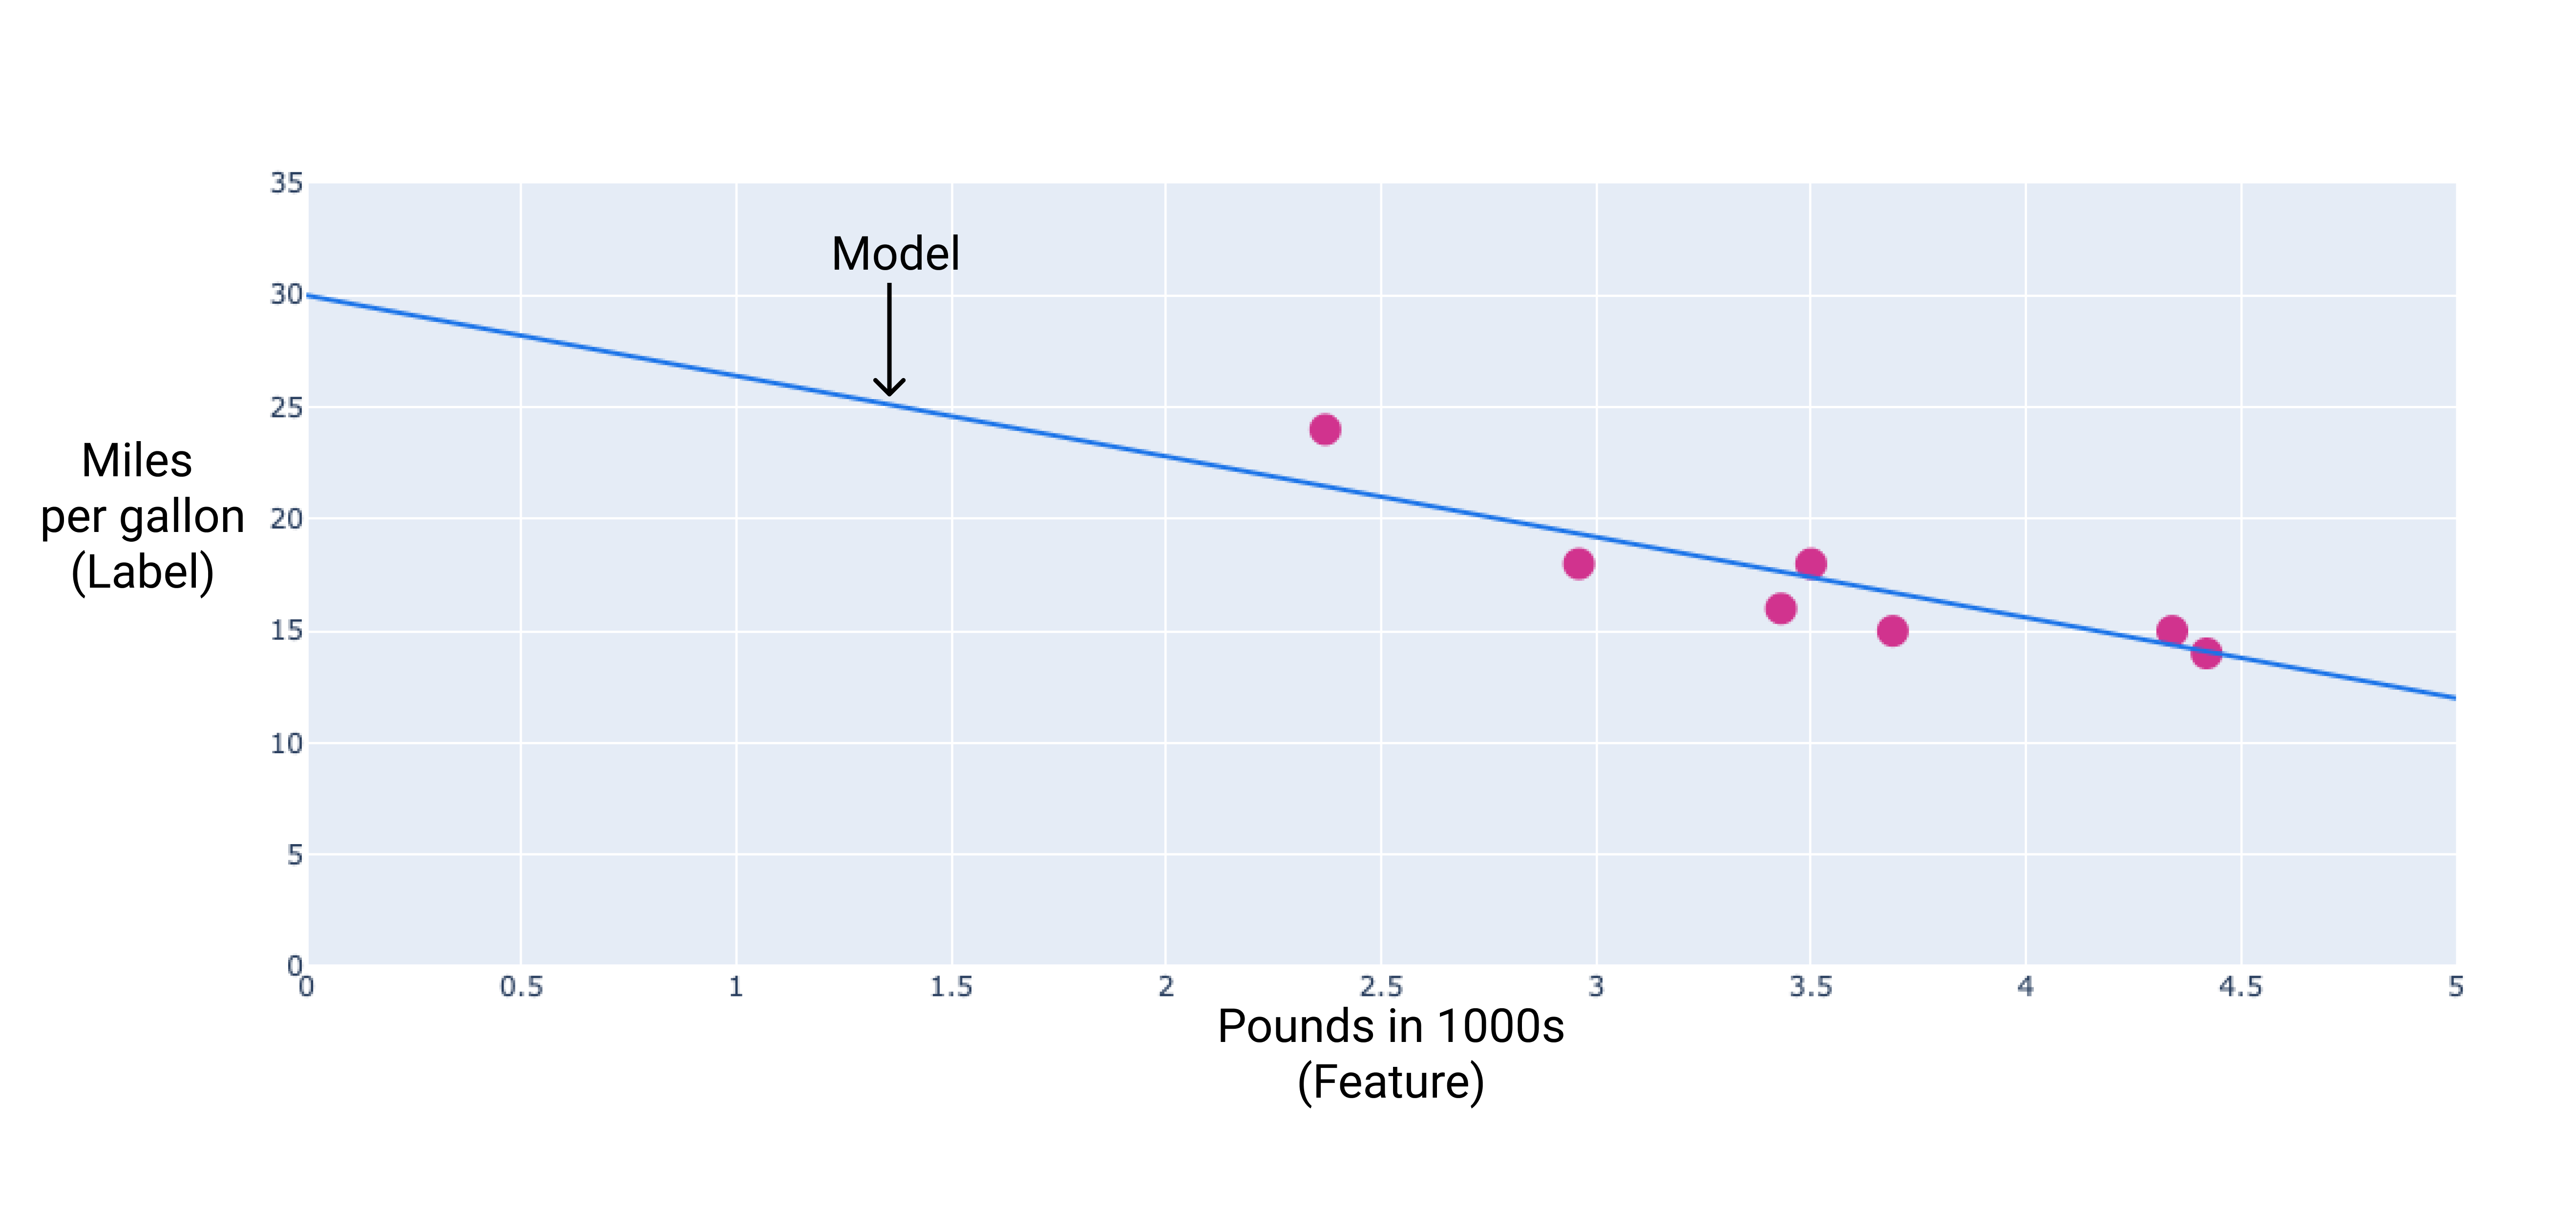
\includegraphics[width=0.7\textwidth]{../Images/Linear-Regression/linear-regression-plot.png}
    \caption{Linear Regression Plot}
    \label{fig:linear-regression-plot}
\end{figure}

\subsection{Linear Regression Equation}

\begin{equation}
\hat{y} = b + w_1 x_1
\end{equation}

\noindent where:

$\hat{y}$: predicted label (output)

$b$: bias/parameter is same as the y-intercept in algebra (shifts the line vertically)
 
$w_1$: weight/parameter is same as the slope $m$ in algebra (steepness of the line)

$x_1$: feature (input) \newline

\noindent During training, the model calculates the $w_1$ and $b$ that produce the best model.

\subsection{Models with Multiple Features}
\begin{equation}
\hat{y} = b + w_1 x_1 + w_2 x_2 + \dots + w_n x_n
\end{equation}

\noindent $x_1, \dots, x_5$ = \{Pounds, Displacement, Acceleration, Number of Cylinders, Horsepower\}

\begin{figure}[H]
    \centering
    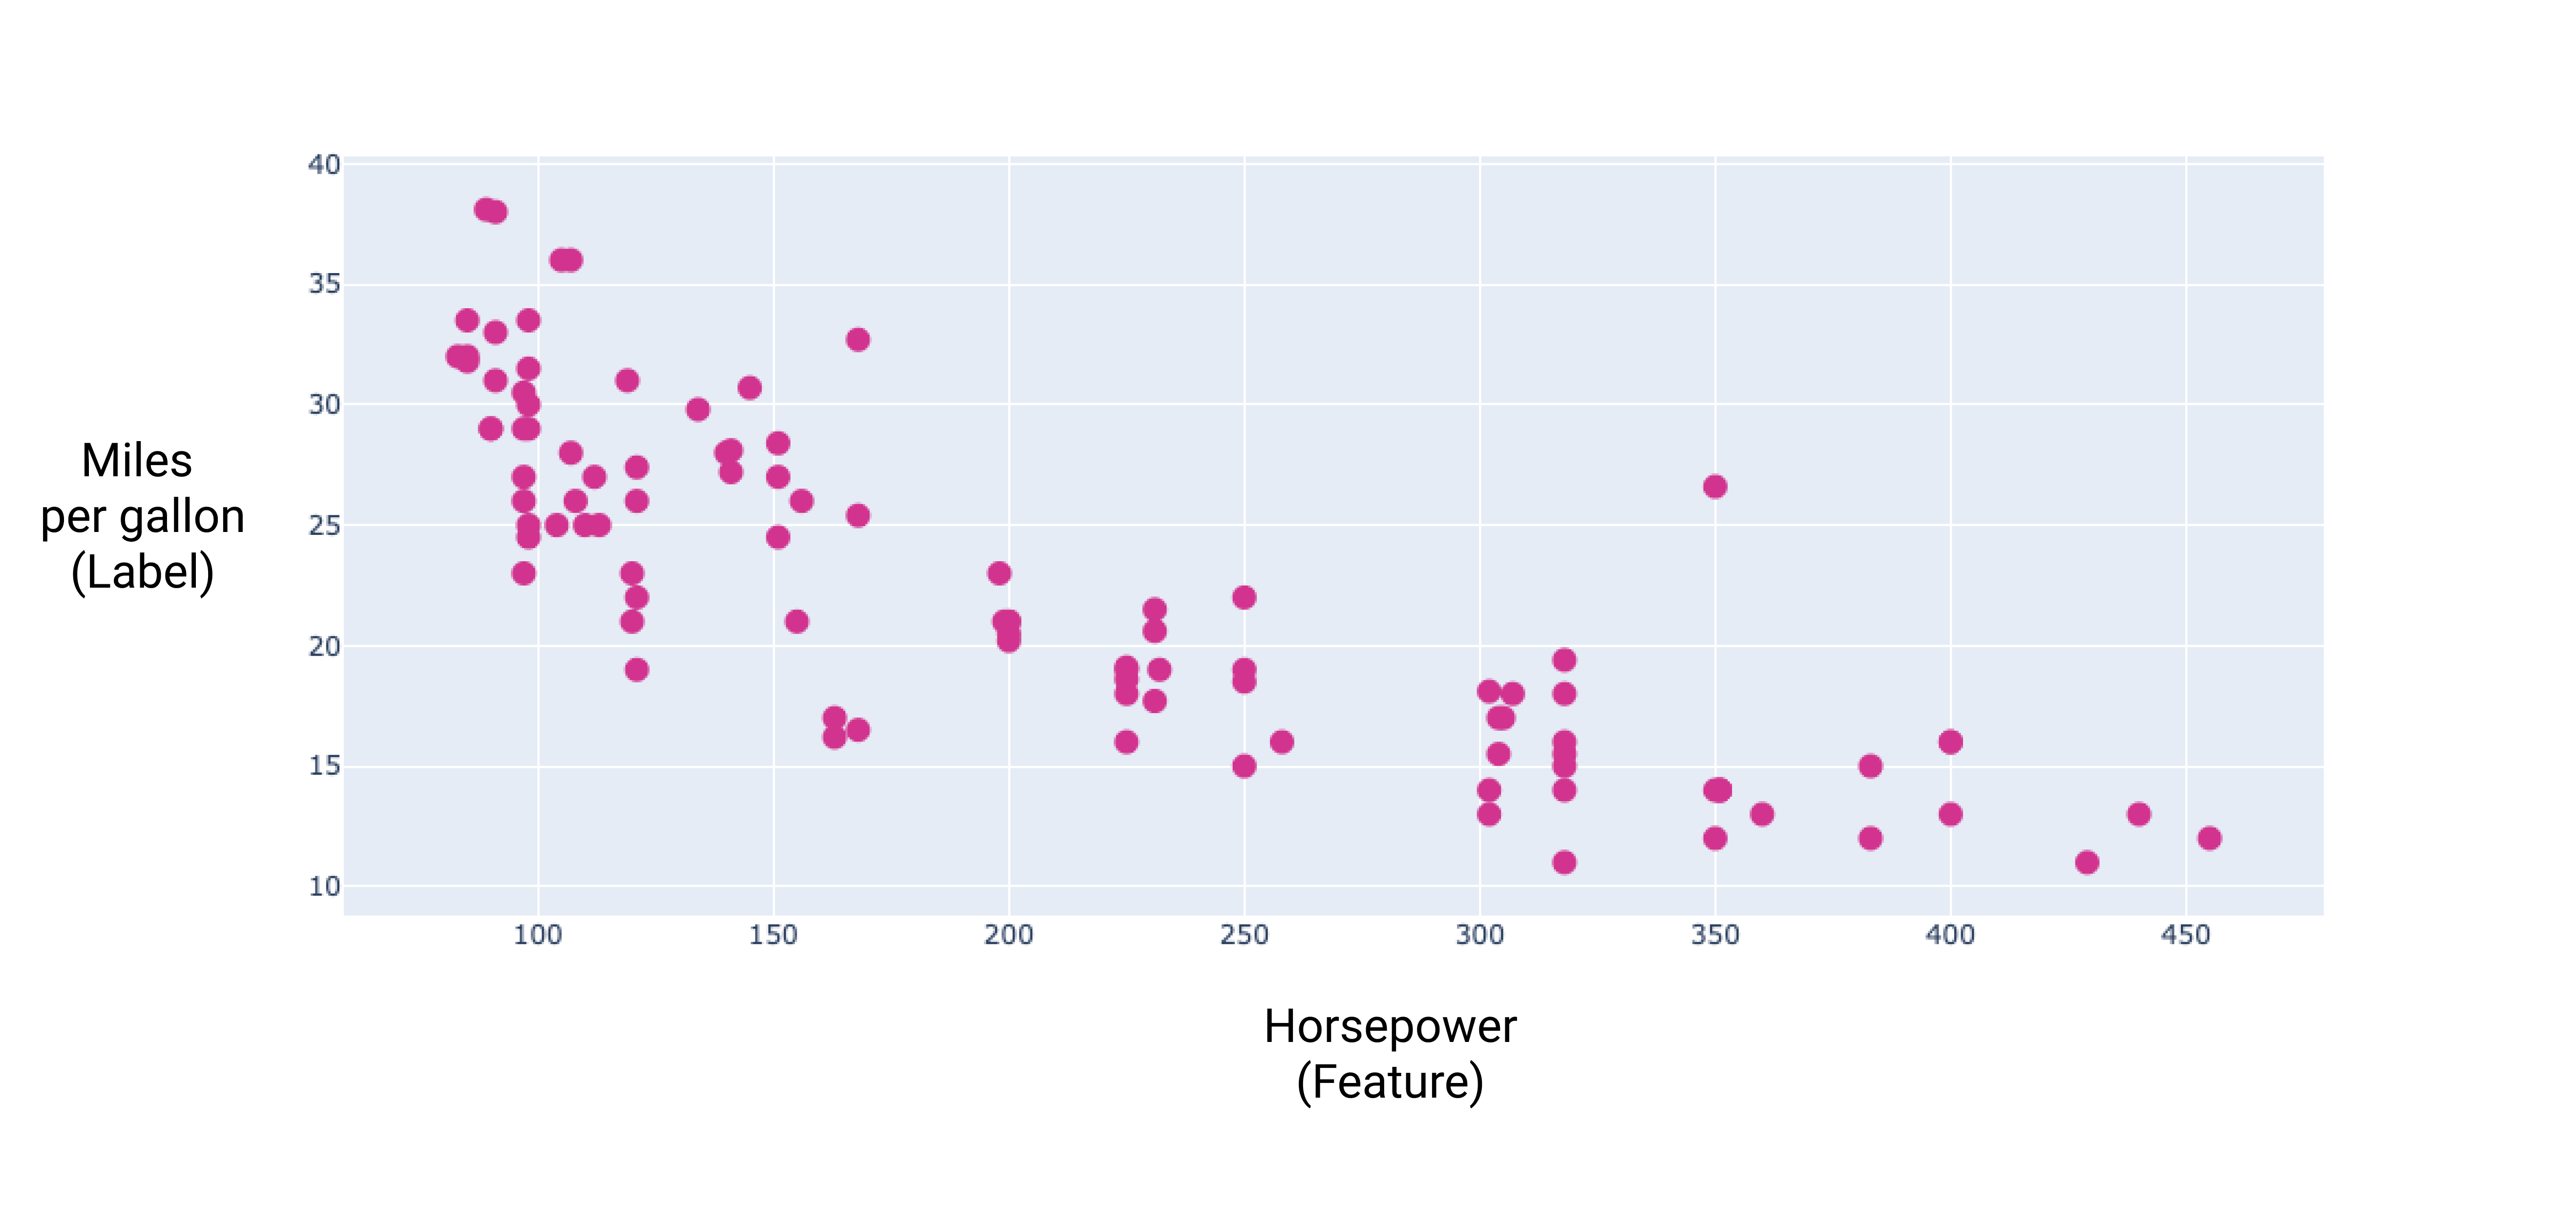
\includegraphics[width=0.7\textwidth]{../Images/Linear-Regression/horsepower-plot.png}
    \caption{Horsepower Plot}
    \label{fig:horsepower-plot}
\end{figure}

\section{Loss Function}
A metric that describes how wrong a model's predictions are. It measures the distance between the model's predictions and the actual values. The objective is to minimize the loss, making it to its lowest possible value.

\begin{figure}[H]
    \centering
    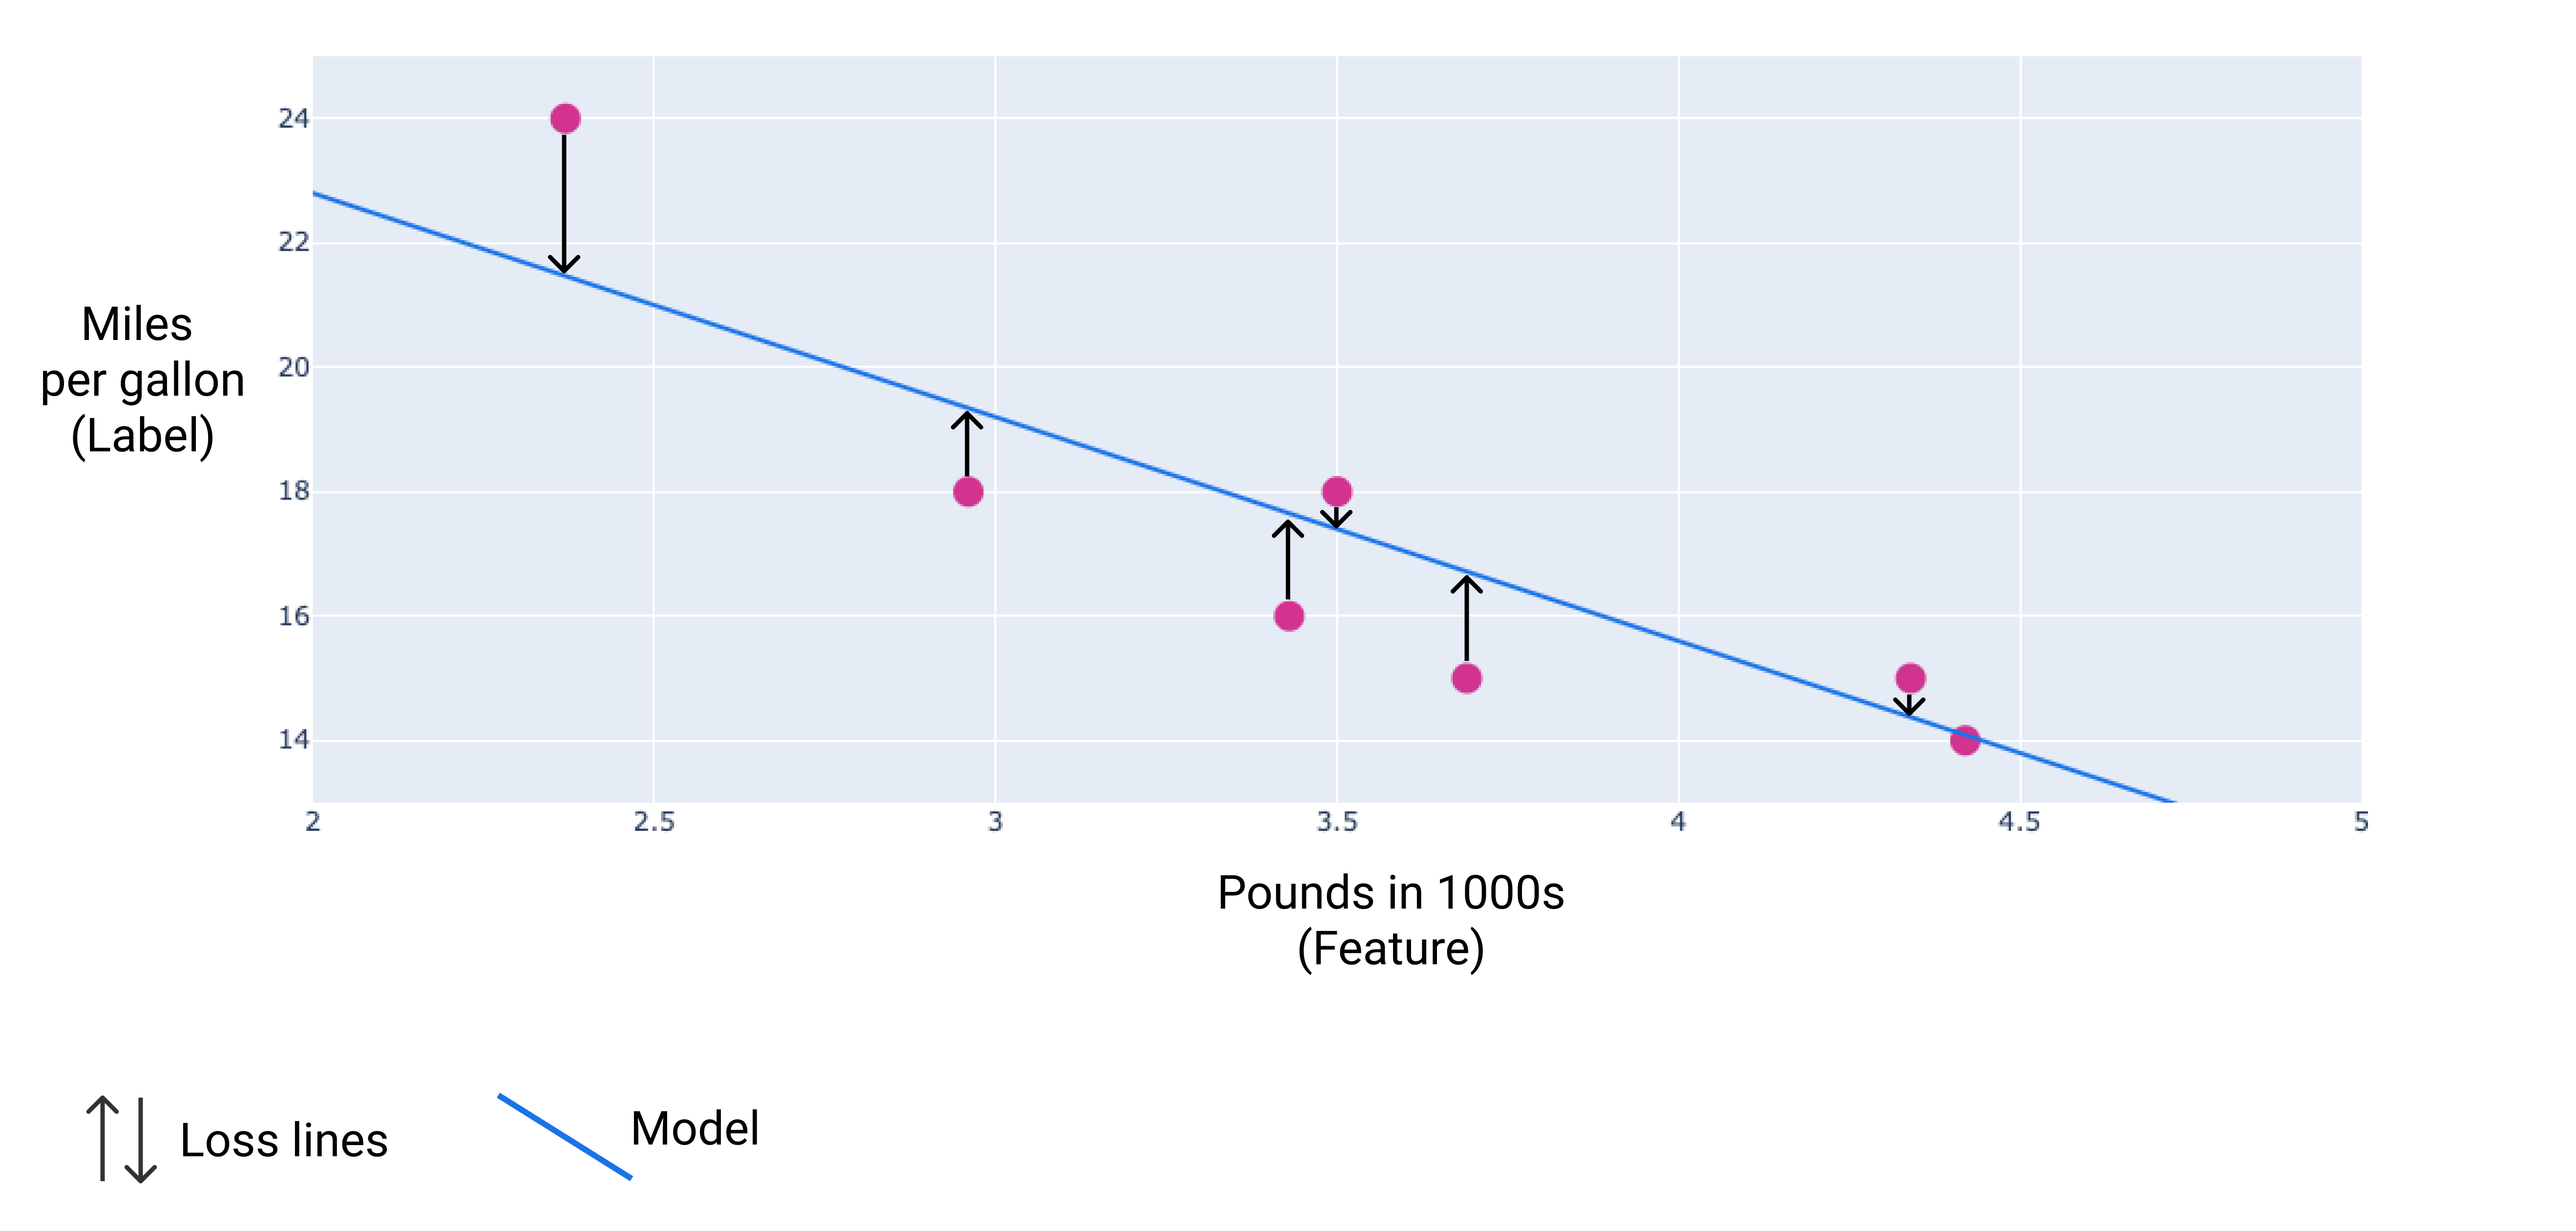
\includegraphics[width=0.7\textwidth]{../Images/Linear-Regression/loss-lines.png}
    \caption{Loss Lines}
    \label{fig:loss-lines}
\end{figure}

\subsection{Distance of Loss}
Loss focuses on the distance, not the value. If the difference is a negative value, we need to remove the sign.

\noindent Common methods to remove the sign: 
\begin{itemize}
    \item Get the absolute value of the difference of errors
    \item Square the difference of errors
\end{itemize}

\subsection{Error}
The difference between the actual and predicted values
\begin{equation}
error = y - \hat{y}
\end{equation}

\subsection{Types of Loss}
\begin{center}
\begin{tabularx}{\textwidth}{@{}lXl@{}}
\toprule
Loss Type & Definition & Equation ($y$) \\ 
\midrule
$L_1$ loss & Sum of the absolute values of the errors & $\sum |y - \hat{y}|$ \\
$L_2$ loss & Sum of the squared difference of the errors & $\sum (y - \hat{y})^2$ \\
Mean Absolute Error (MAE) & Average of $L_1$ losses across $N$ & $ \frac{1}{N} \sum |y - \hat{y}|$ \\
Mean Squared Error (MSE) & Average of $L_2$ losses across $N$ & $ \frac{1}{N} \sum (y - \hat{y})^2$ \\
\bottomrule
\end{tabularx}
\end{center}

\noindent It is recommended to use MAE or MSE.

\subsection{Loss Calculation Example}
Calculate the $L_2$ loss:

$w_1$: -3.6

$b$: 30

\noindent If a model predicts that a 2,370-pound car gets 21.5 miles per gallon, but it actually gets 24 miles per gallon, then:
\begin{align}
\hat{y} &= b + (w_1 + \text{feature value}) \\
       &= 30 + (-3.6 * 2.37) \\ &= 21.5
\end{align}

\noindent $y$ = 24, $\hat{y}$ = 21.5

\begin{align}
L_2 &= (y - \hat{y})^2 \\
    &= (24 - 21.5)^2 \\
    &= 6.25
\end{align}

\subsection{Choosing a Loss}
An outlier is a value that lies outside the typical range of a dataset. \textbf{Mean Squared Error (MSE)} is more sensitive to outliers, giving them greater influence on the loss. In contrast, \textbf{Mean Absolute Error (MAE)} is less affected by outliers and stays closer to the majority of the data points.


\section{Gradient Descent}
Gradient Descent is an iterative process used to update the weight and bias in order to minimize the loss.
\begin{enumerate}
    \item Initialize the $w$ and $b$ to 0.
    \item Compute the loss function using the current $w$ and $b$.
    \item Compute the gradients of the loss with respect to $w$ and $b$, then update the parameters by moving them a small step in the direction that decreases the loss (using the learning rate).
    \item Repeat steps 2 and 3 until convergence (when the loss stops decreasing significantly or after a set number of iterations).
\end{enumerate}

\subsection{Math Behind Gradient Descent}
Pounds in 1000s = [3.5, 3.69, 3.44, 3.43, 4.34, 4.42] \newline
Miles per gallon = [18, 15, 18, 16, 15, 14, 24] \newline

\noindent 1. Initialize the $w$ and $b$ to 0.
\begin{align}
w &= 0 \\
b &= 0 \\
\hat{y} &= 0 + 0(x_1)
\end{align}

\noindent 2. Calculate MSE loss with current model parameters
\begin{align}
\text{MSE} &= \frac{(18-0)^2 + (15-0)^2 + (18-0)^2 + (16-0)^2 + (15-0)^2 + (14-0)^2 + (24-0)^2}{7} \\
 &= 303.71
\end{align}

\noindent 3. Calculate the slope of the tangent to the loss function at each weight and the bias
\begin{align}
\text{w slope} &= -119.7 \\
\text{b slope} &= -34.3
\end{align}

\textbf{How?} Derivatives... \newline

\noindent 4. Move a small amount (learning rate: 0.01) in the direction of the negative slope to get the next $w$ and $b$.
\begin{align}
w &= w - (0.01 * -119.7) \\
b &= b - (0.01 * -34.3) \\
w_{\text{new}} &= 1.2 \\
b_{\text{new}} &= 0.34 \\
\end{align}

\begin{table}[h!]
\centering
\begin{tabular}{|c|c|c|c|}
\hline
\textbf{Iteration} & \textbf{Weight} & \textbf{Bias} & \textbf{Loss (MSE)} \\
\hline
1 & 0.00 & 0.00 & 303.71 \\
2 & 1.20 & 0.34 & 170.67 \\
3 & 2.75 & 0.59 & 67.30 \\
4 & 3.17 & 0.72 & 50.63 \\
5 & 3.47 & 0.82 & 42.10 \\
6 & 3.68 & 0.90 & 37.74 \\
\hline
\end{tabular}
\caption{Training Progress Over Iterations}
\label{tab:training_progress}
\end{table}

Continue training until the loss has stabilized.

\subsection{Loss Curves}
The loss curve shows how the loss changes as the model trains. 
\begin{itemize}
    \item \textbf{x-axis}: iterations 
    \item \textbf{y-axis}: loss
\end{itemize}

\begin{figure}[H]
    \centering
    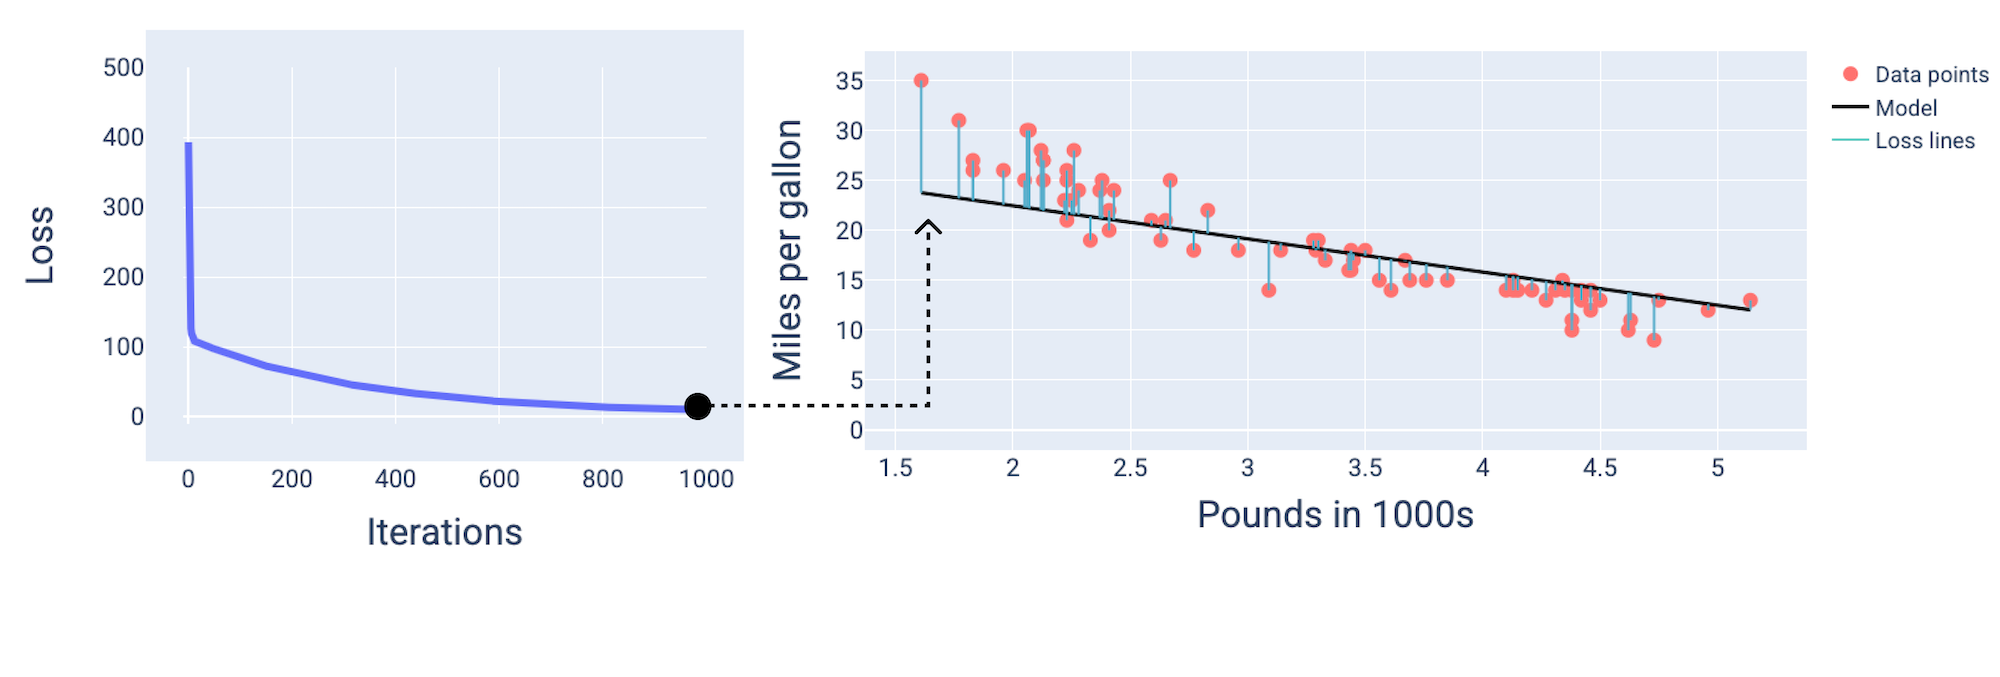
\includegraphics[width=0.7\textwidth]{../Images/Linear-Regression/low-loss.png}
    \caption{Low Loss Curve}
    \label{fig:low-loss}
\end{figure}

\subsection{Convergence and Convex Functions}
The loss functions for \textbf{linear models} always produce a \textbf{convex} surface. 
\begin{itemize}
    \item \textbf{x-axis}: weight
    \item \textbf{y-axis}: bias 
    \item \textbf{z-axis}: loss 
\end{itemize}
\begin{figure}[H]
    \centering
    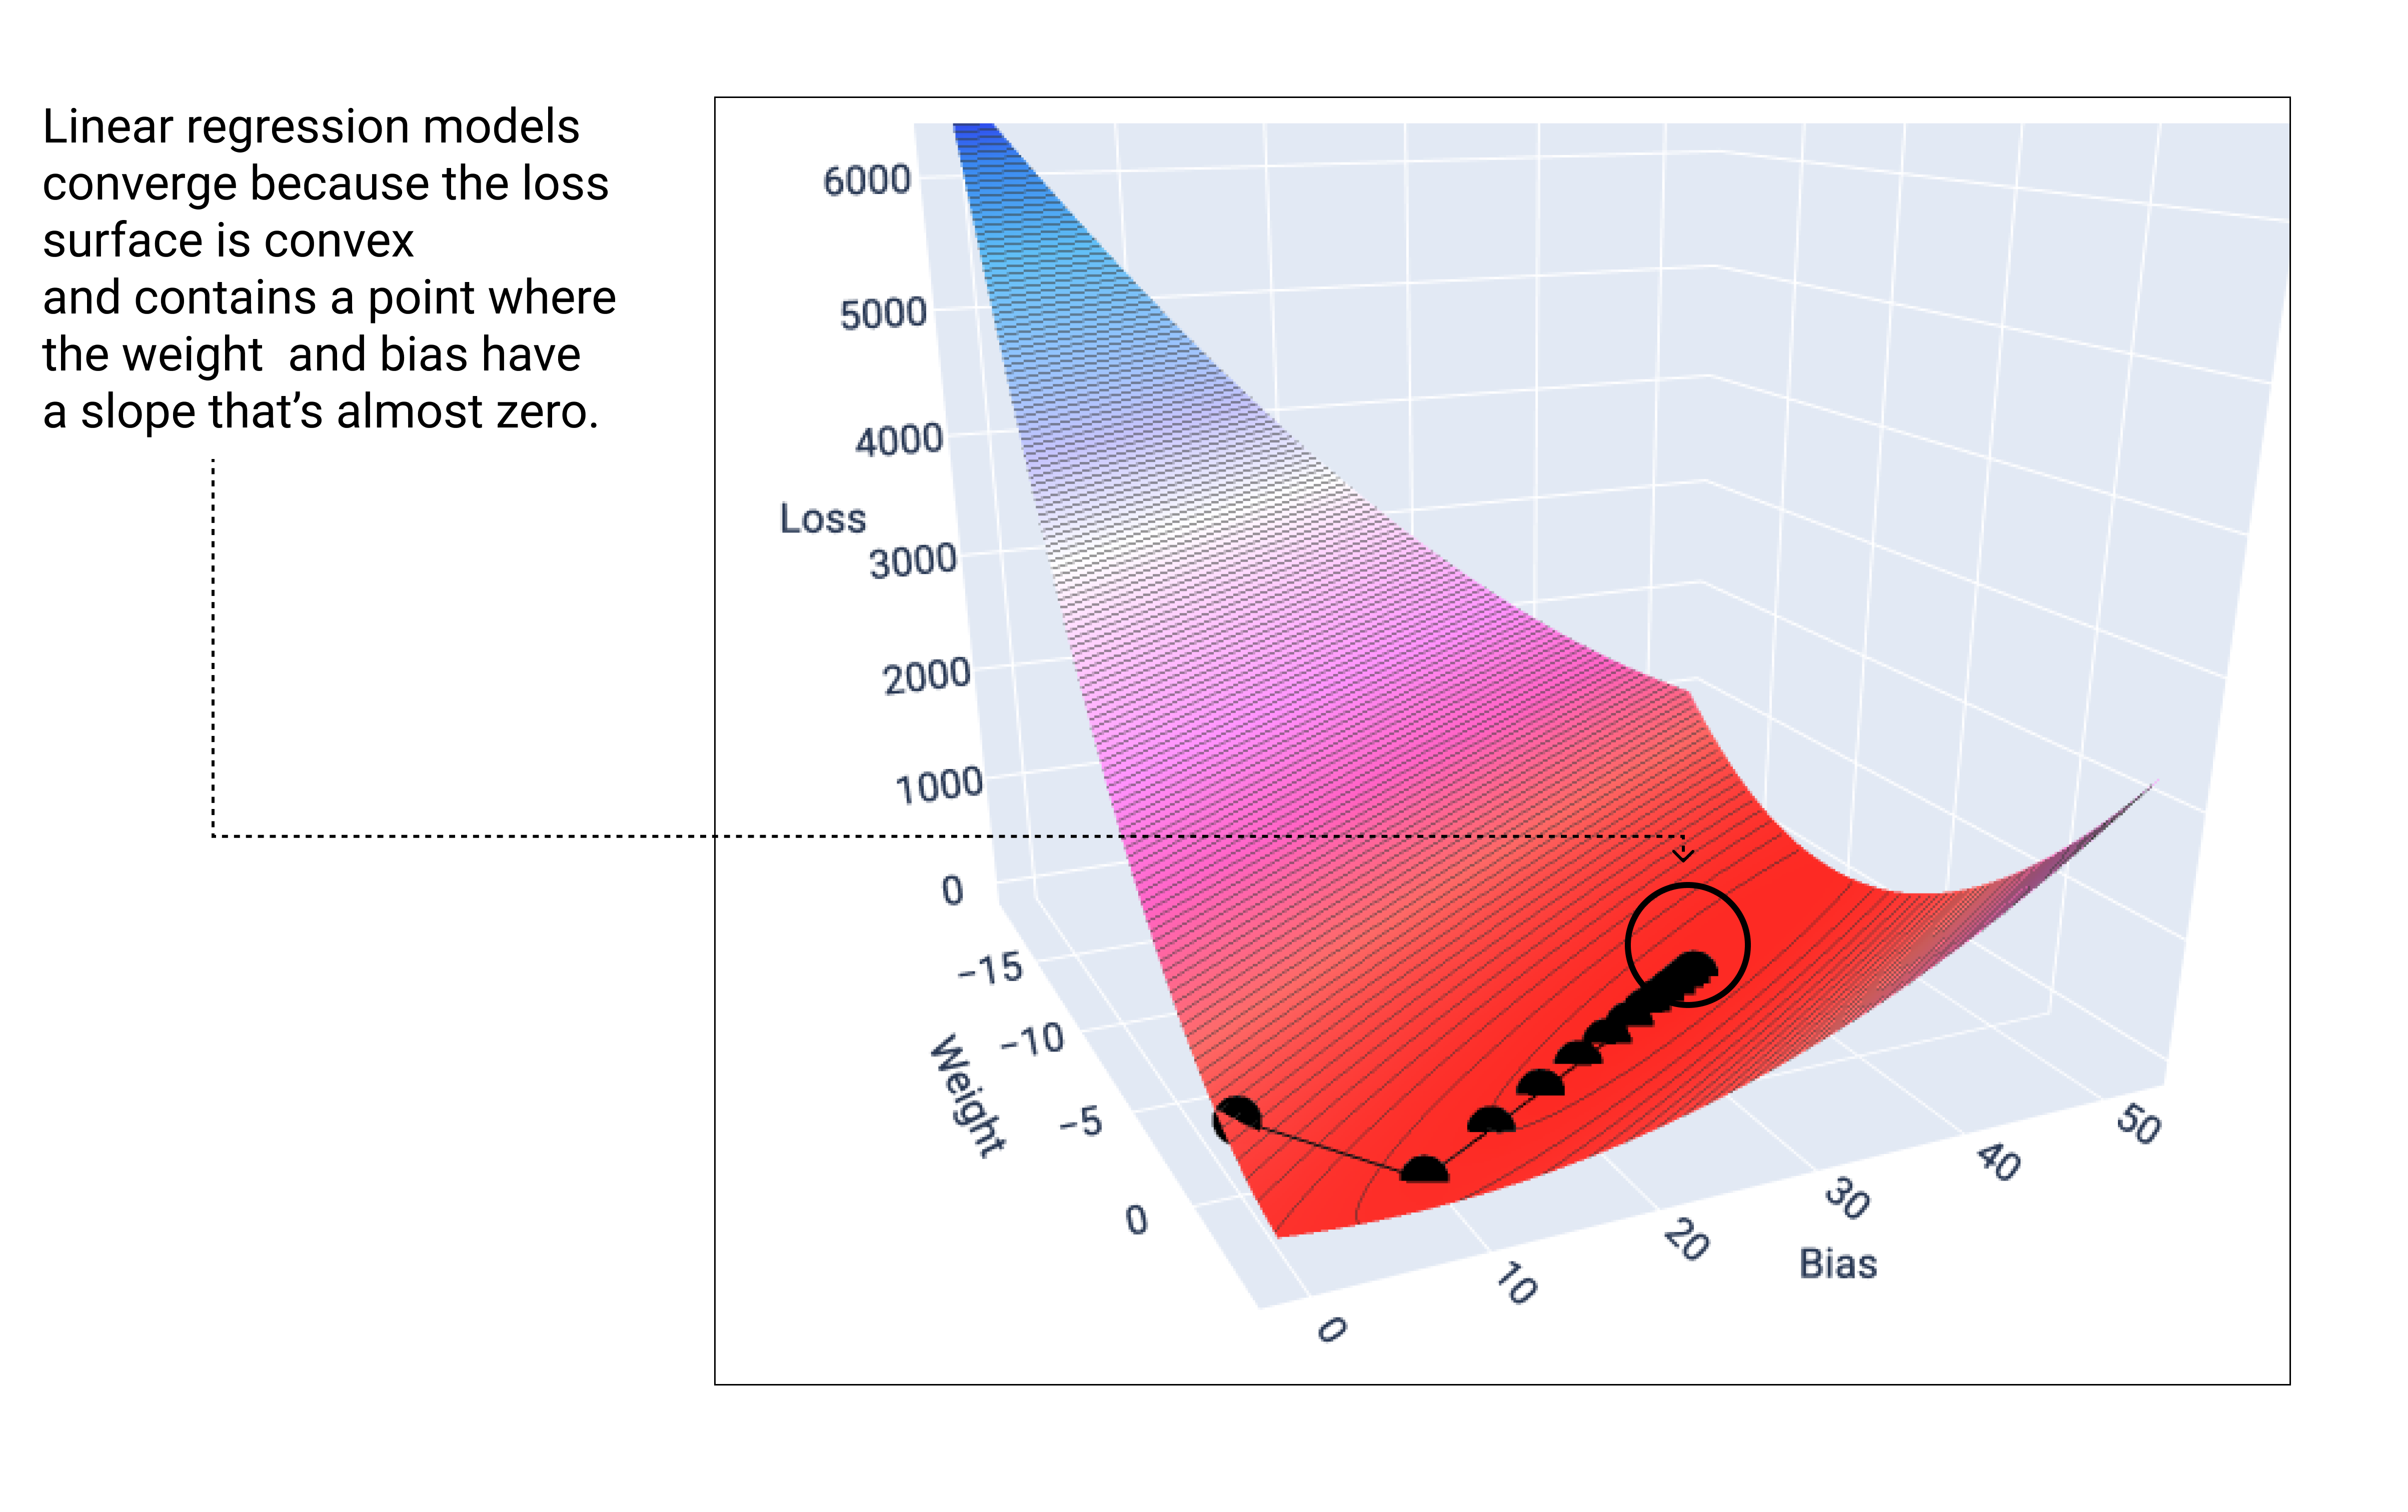
\includegraphics[width=0.7\textwidth]{../Images/Linear-Regression/loss-surface-points.png}
    \caption{Loss Surface Points}
    \label{fig:loss-surface}
\end{figure}

A linear model converges when it reaches the point of minimum loss. After this, further iterations cause only minor adjustments to the weights and bias. This process is like a ball rolling downhill and settling at the lowest point. While the model may not find the exact minimum, it gets very close. Importantly, this minimum doesn't mean zero loss—just the lowest possible loss for the given parameters. It will never reach zero, but close to zero. 0.00310

\section{Hyperparameters}
\textbf{Hyperparameters} are values that you control. \textbf{Parameters} are values that the model calculates during training.

\subsection{Learning Rate}
It influences how quick the model converges. \newline
\textbf{Learning rate: too low} - the model will take a long time to converge. \newline
\textbf{Learning rate: too high} - the model may never converge and will bounce around the values of $w$ and $b$ that minimize the loss. \newline
\textbf{Common learning rates}: \{0.1, 0.01, 0.001, 0.0001\}, depending on the model and dataset.

\begin{figure}[H]
    \centering
    \begin{subfigure}[b]{0.45\textwidth}
        \centering
        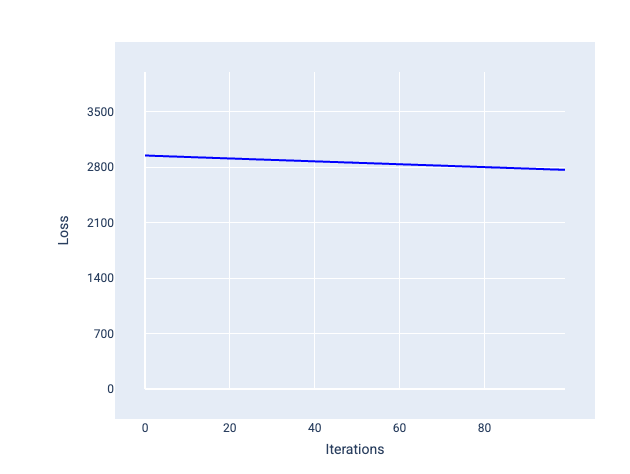
\includegraphics[width=\textwidth]{../Images/Linear-Regression/small-lr.png}
        \caption{Small Learning Rate}
        \label{fig:small-lr}
    \end{subfigure}
    \hfill
    \begin{subfigure}[b]{0.45\textwidth}
        \centering
        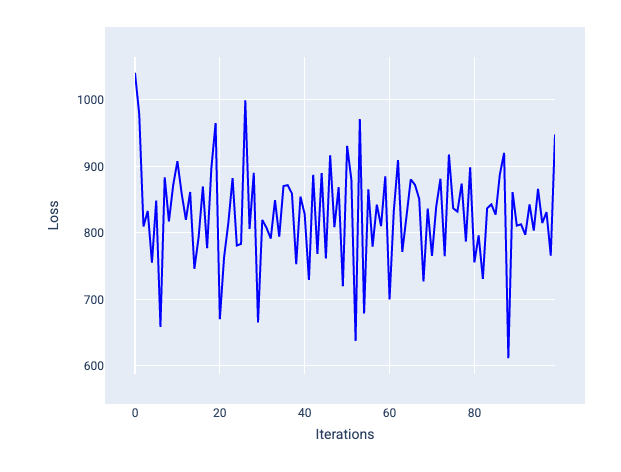
\includegraphics[width=\textwidth]{../Images/Linear-Regression/high-lr.png}
        \caption{Large Learning Rate}
        \label{fig:large-lr}
    \end{subfigure}
    \begin{subfigure}[c]{0.45\textwidth}
        \centering
        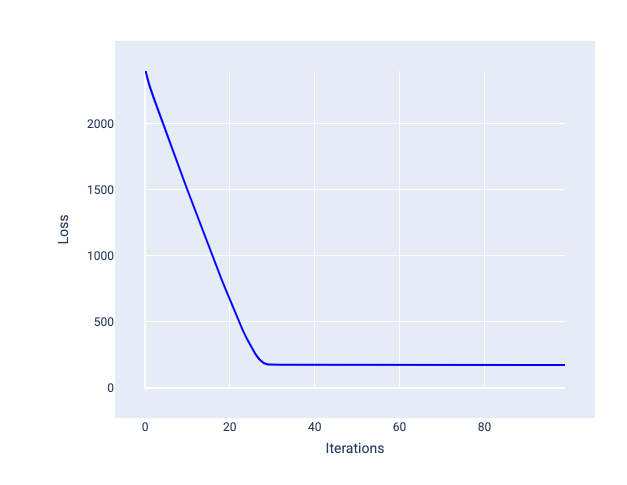
\includegraphics[width=\textwidth]{../Images/Linear-Regression/correct-lr.png}
        \caption{Correct Learning Rate}
        \label{fig:correct-lr}
    \end{subfigure}
    \caption{Comparison of Learning Rates}
    \label{fig:lr-comparison}
\end{figure}

\subsection{Batch Size}
Number of examples the model processes before updating its $w$ and $b$. When a dataset contains thousands 
or even millions of examples, using the full batch isn't practical.
\subsubsection{Stochastic Gradient Descent (SGD)} 
Uses only a single example (a batch size of one) per iteration. One example comprising each batch is chosen at random. It is \textbf{Noisy}. "Noise" refers to variations during training that cause the loss to increase rather than decrease during an iteration. 
\begin{figure}[H]
    \centering
    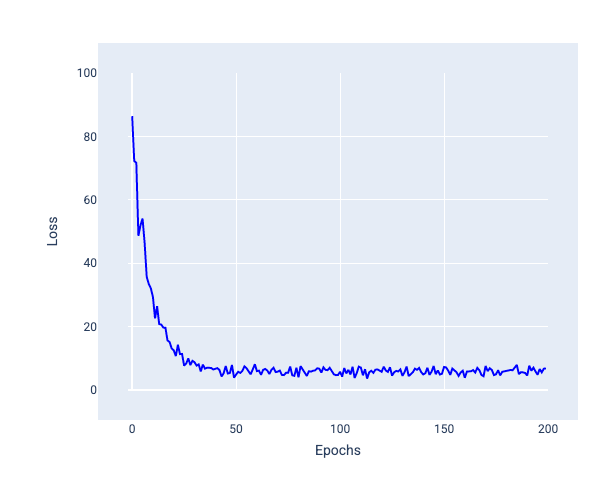
\includegraphics[width=0.7\textwidth]{../Images/Linear-Regression/noisy-gradient.png}
    \caption{Stochastic Gradient Descent}
    \label{fig:noisy-gradient}
\end{figure}


\subsubsection{Mini-batch Stochastic Gradient Descent (mini-batch SGD)}
For $N$ number of data points, the batch size is between 1 and $N-1$.  The model chooses the examples included in each batch at random, averages their gradients, and then updates the weights and bias once per iteration.

\begin{figure}[H]
    \centering
    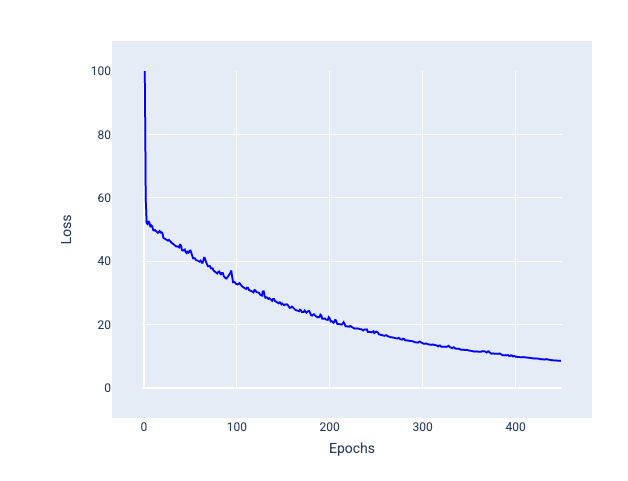
\includegraphics[width=0.7\textwidth]{../Images/Linear-Regression/mini-batch-sgd.png}
    \caption{Mini-batch Stochastic Gradient Descent}
    \label{fig:mini-batch-sgd}
\end{figure}

\subsection{Epochs}
It means that the model has processed every example in the training set once. More epochs produces a better model, but also takes more time to train.

\begin{center}
\begin{tabularx}{\textwidth}{@{}lXl@{}}
\toprule
Batch Type & When parameters update occur \\ 
\midrule
Full batch & Updates weights once per epoch after using the entire dataset  \\
Stochastic Gradient Descent & Updates weights after each individual example \\
Mini-batch SGD & Updates weights after each mini-batch of examples \\
\bottomrule
\end{tabularx}
\end{center}

\begin{figure}[H]
    \centering
    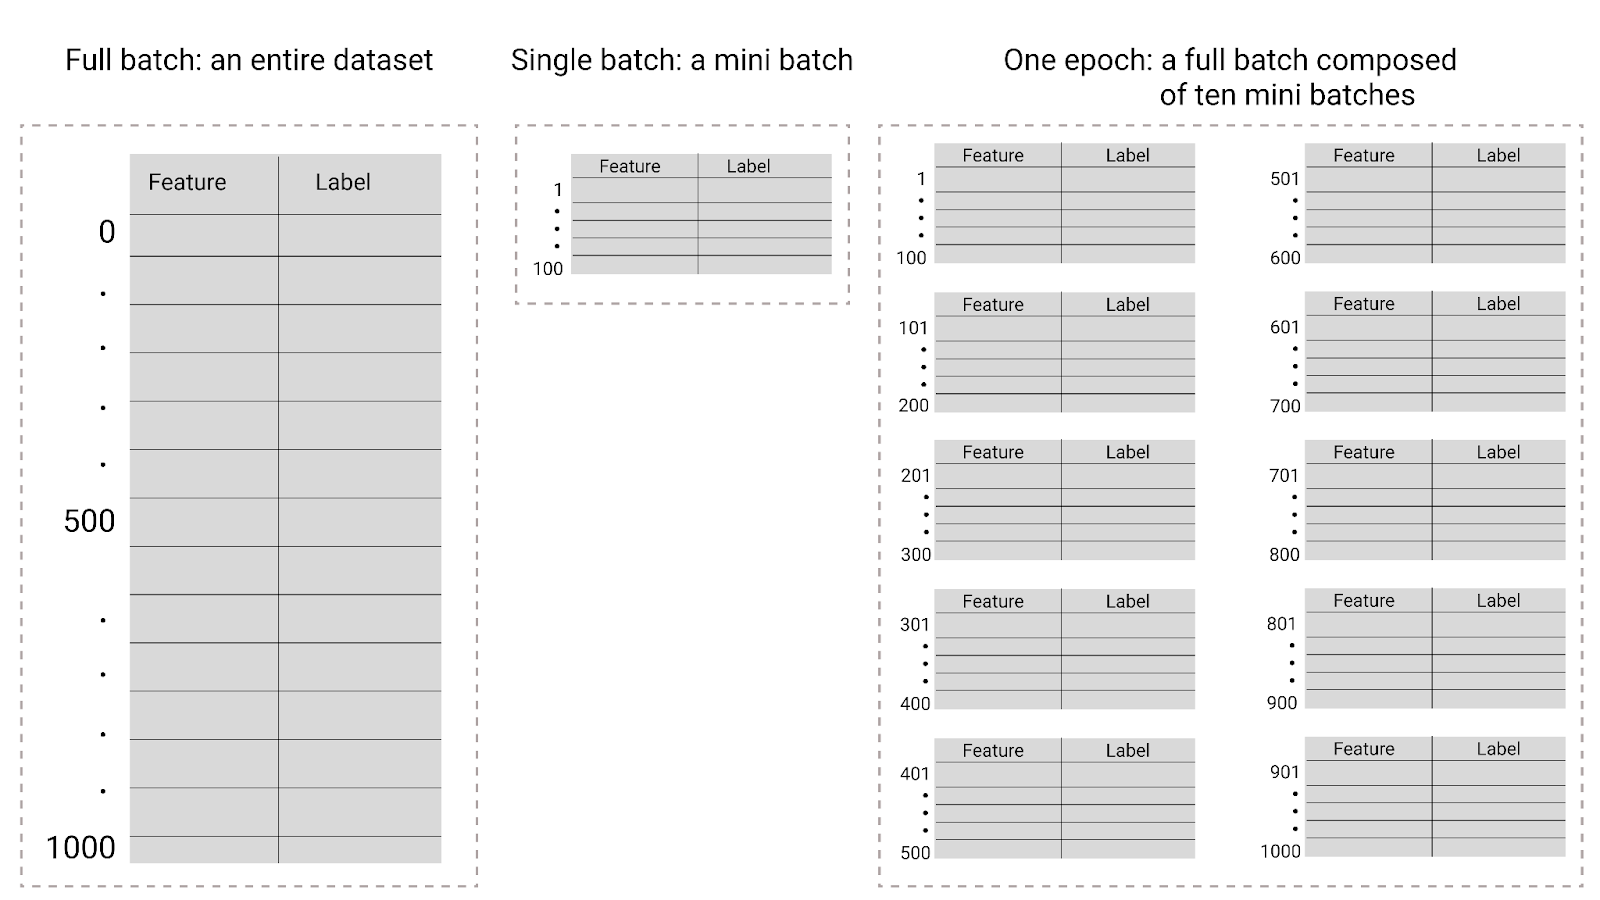
\includegraphics[width=0.7\textwidth]{../Images/Linear-Regression/batch-size.png}
    \caption{Full batch versus mini-batch}
    \label{fig:batch-size}
\end{figure}

\section{References}
\begin{itemize}
    \item \href{https://developers.google.com/machine-learning/crash-course/linear-regression}{Linear Regression - Google Developers}
    \item \href{https://developers.google.com/machine-learning/glossary}{Machine Learning Glossary - Google Developers}
\end{itemize}


\end{document}
